\chapter{Critical Angle}

\section{Aim}
To determine the critical angle of light passing from glass into air by using a semicircular glass block

\section{Background Information}
Light bends when it passes from one medium to another. Perhaps there is a special angle of incidence at which light bends beyond $90^\circ$ so that it would actually reflect. The critical angle is when the angle of refraction is $90^\circ$ and this reflection begins. If this angle is exceeded then internal reflection can occur. This is useful for controlling light and a common application is high-speed internet cables called optical fibers. Fiber optics use internal reflection of light to transfer computer signals from one place to another. Therefore, it is important to know how to find the critical angle.

\section{Materials}
Semicircular glass block, ray box, drawing pin, white sheet of paper, protractor, pencil, meter rule and drawing board

\section{Procedure}
\begin{enumerate}
\item Fix a sheet of white paper on a drawing board using drawing pins.
\item Place a semicircular glass block at the center of the white sheet of paper.
\item Trace the outline of the semicircular block on the paper using a pencil.
\item Remove the semicircular glass block and mark the point O on the paper at the middle of the line on the flat side of the block. 
\item Use a protractor to draw a line through point O which is perpendicular to the line of the flat side of the block.  Label this line MN.
\item Use the protractor to draw 7 different lines which make an angle $i$ of $20^\circ$, $36^\circ$, $38^\circ$, $42^\circ$, $44^\circ$, $46^\circ$, and $48^\circ$ with the line ON. Label the lines as I$_1$, I$_2$ \ldots I$_7$ respectively.
\item Place the semicircular glass block back into its original position within the outline drawn in step (3).
\item Place the ray box so that the emitted ray follows line I$_1$. Using a ruler, trace the line which exits the glass block from the flat side. Label it R$_1$. 
\item Observe and record the brightness of the refracted and reflected rays.
\item Repeat steps (8) and (9) for the other 6 lines and label each ray exiting the flat side accordingly.
\item Remove the semicircular glass block and use the protractor to measure the angles of refraction, $r$, and record them in tabular form. If no ray exited the flat side, insert ‘no ray’ into the table.
\end{enumerate}

\begin{figure}[h!]
\centering
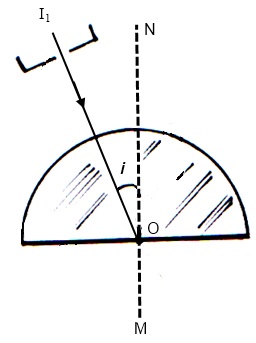
\includegraphics[width=4cm]{./img/critical-angle-1}
\caption{Critical Angle practical setup}
\label{fig:critical-angle-1}
\end{figure}

%\section{Safety Measure}
%The experiment should be carried out in a darkened room.

\section{Analysis and Interpretation}
\begin{enumerate}
\item What general trend do you observe in the refracted angle as the incident angle increases?
\item At what angle of incidence does the angle of refraction go to $90^\circ$? 
\item What did you observe after this angle? 
\item What is the trend in brightness of the refracted ray before the angle found in question 2? Comment on this observation.
\item What is the trend in brightness of the \emph{reflected} ray after the angle found in question 2? Comment on this observation.
\item Calculate the index of refraction of the glass block using your experimental results before the angle found in question 2. Use this value to calculate the critical angle of glass into air. 
\end{enumerate}

\section{Conclusion}
From the experiment, what is the critical angle of this semicircular glass block into air?

\section{Questions for Discussion}
\begin{enumerate}
\item Why did we use a semicircular glass block in this experiment and how might the use of another shape have been more difficult to use?
\item Explain the possible errors in this experiment. How do they affect your results?
\item Do you predict there will be a critical angle for light moving from air into glass? Support your explanation mathematically.
\item How might a person constructing a diamond ring use internal reflection to make the diamond more beautiful so that he can sell it at a higher price?
\end{enumerate}

\section{Reflection and Self Assessment}
\begin{enumerate}
\item Do you understand everything in this experiment? If not, what can you do to increase your understanding?
\item What were the most and least interesting parts of this experiment to you? Explain.
\end{enumerate}